% gjilguid2e.tex
% V2.0 released 1998 December 18
% V2.1 released 2003 October 7 -- Gregor Hutton, updated the web address for the style files.

\documentclass{gji}
\usepackage{timet,color}
\usepackage{graphicx} 
 \usepackage{geometry}
% \geometry{paperwidth=8.5in, paperheight=11in}
% \geometry{paperheight=11in}
\usepackage[urlcolor=blue,citecolor=black,linkcolor=black]{hyperref}
\graphicspath{{figs/}}
%\usepackage[numbers]{natbib}
\usepackage[authoryear]{natbib}
% \usepackage{siunitx}
\usepackage{enumerate}
\usepackage{multirow}
\usepackage{adjustbox}
\usepackage{booktabs, csquotes}
\usepackage{float}
\usepackage{caption}
\usepackage{subcaption}
\usepackage{placeins}  % For \FloatBarrier
% \numberwithin{figure}{section}
% \numberwithin{table}{section}
% \usepackage{threeparttable}
\usepackage{amsmath}	% Advanced maths commands
\usepackage{amssymb}
% \sloppy 


\title[Analysis of Well-C in the Offshore Keta Basin]
  {Analysis of Well-C in the Offshore Keta Basin: Petrophysical Examination}
% \author[H. Adams {\rm et~al.}]
%   {Hamdiya Adams$^1$\thanks{Pacific Region Office, GJI,
%    } \\
%   $^1$ Research School of Earth Sciences, Australian National
%     University, Canberra ACT \emph{0200}, Australia
%   }
\author[H. Adams {\rm et~al.}]{
Hamdiya Adams$^{1}$,
Theophilus Ansah-Narh$^{2}$\thanks{E-mail: \href{theophilus.ansah-narh@gaec.gov.gh}{theophilus.ansah-narh@gaec.gov.gh} (TA-N)},
Daniel K. Asiedu$^{1}$,
\and
Bruce K. Banoeng-Yakubo$^{1}$,
Thomas Armah$^{1}$,
and Mustapha Odainkey$^{3}$
\\
% List of institutions
$^{1}$Department of Earth Science, University of Ghana, P. O. Box LG 58, Legon-Accra, Ghana\\
$^{2}$Ghana Space Science \& Technology Institute, Ghana Atomic Energy Commission, P. O. Box LG 80, Legon-Accra, Ghana\\
$^{3}$Petroleum Commission, Plot No. 4A, George Bush Highway, Accra, Ghana
}

% \author[B.L.N. Kennett]
%    {B.L.N. Kennett$^1$
%   \thanks{Pacific Region Office, GJI} \\
%   $^{1}$Research School of Earth Sciences,
%     Australian National University,
%     Canberra ACT \emph{0200}, Australia, \\
%     B.L.N. Kennett$^1$ \\
%   $^{1}$Research School of Earth Sciences,
%     Australian National University,
%     Canberra ACT \emph{0200}, Australia
%   }
\date{Received 1998 December 18; in original form 1998 November 22}
\pagerange{\pageref{firstpage}--\pageref{lastpage}}
\volume{200}
\pubyear{1998}

%\def\LaTeX{L\kern-.36em\raise.3ex\hbox{{\small A}}\kern-.15em
%    T\kern-.1667em\lower.7ex\hbox{E}\kern-.125emX}
%\def\LATeX{L\kern-.36em\raise.3ex\hbox{{\Large A}}\kern-.15em
%    T\kern-.1667em\lower.7ex\hbox{E}\kern-.125emX}
% Authors with AMS fonts and mssymb.tex can comment out the following
% line to get the correct symbol for Geophysical Journal International.
\let\leqslant=\leq

\newtheorem{theorem}{Theorem}[section]

\begin{document}

\label{firstpage}

\maketitle


\begin{summary}
 In Ghana, there exist four sedimentary basins, one of which is the Keta basin, a relatively underexplored region. 
The primary objective of the study goes beyond merely estimating pivotal petrophysical parameters essential for hydrocarbon exploration; it extends to the precise delineation of reservoir zones.
This analytical pursuit is deemed necessary due to the limited number of exploratory wells within the basin.
A variety of well logs, including gamma-ray, resistivity, density, and neutron, have been harnessed for this investigation.
These logs serve as valuable tools in ascertaining the lithological composition of the region, primarily comprising sand, shale, and trace amounts of limestone.
The reservoir zone, situated in the Cenomanian with a total thickness of 164.28 meters, has been further categorized into Lower Cenomanian Sand, Top Cenomanian Sand 1, and Top Cenomanian Sand 2.
The lithological characterisation of the reservoir was achieved through a cross-plot analysis of density and neutron logs, revealing predominantly sandstones with minimal traces of limestone. Shale content within the reservoir varies from $2.4\%$ to $18.2\%$. 
Furthermore, the water saturation levels exhibit a range of 72\% to 86\%, while porosity values fall within the range of 11\% to 13\%.
Despite these detailed findings, the presence of tight sands in Well-C suggests that, at present, the reservoir may not be economically viable for the sufficient generation of hydrocarbons.
However, it is crucial to acknowledge that diverse outcomes may emerge from future studies, especially if additional data sources, such as seismic data and an expanded well dataset are incorporated into the analysis.
\end{summary}

\begin{keywords}
 Composition and structure of the continental crust, Fault zone rheology, Fracture and flow, Sedimentary basin processes, Permeability and porosity,
\end{keywords}

\section{Introduction}

Petrophysical analysis is an intriguing exploration of the world hidden beneath the Earth's surface and is a diverse field that explores the complex system between rocks and fluids.
This field of research, which was originally introduced by \cite{archie1950introduction}, includes the study of physical, chemical, and hydrodynamic properties through the interpretation of well logs \citep{mondol2015well,buryakovsky2012fundamentals,glover2000petrophysics}.
Well logging serves as a crucial instrument in the acquisition of physical measurements during the exploration phase of hydrocarbons. 
This indispensable technique involves the recording and analysis of various parameters within a borehole to gather valuable data regarding subsurface formations.
By employing well logging, exploratory efforts gain insights into geological characteristics such as rock composition, porosity, permeability, radioactivity, density, resistivity, and fluid content, all of which are vital in assessing the potential presence and viability of hydrocarbon reservoirs \citep{ellis2007well,Tittman2012,liu2017principles}. 

A recent study by \cite{das2018well} focused on well log analysis in the Krishna-Godavari basin, examining six wells to derive information about the petrophysical properties (like volume of shale, effective porosity, and water saturation) and fluid content of reservoir rocks. 
Various logs, including gamma-ray, resistivity, density, and neutron logs, were interpreted for lithology and identification of hydrocarbon-bearing zones.
The gamma-ray log reveals sediment deposition trends, while gas-bearing zones are characterized by low gamma-rays, high deep resistivity, and crossover between neutron and density logs. 
Another study by \cite{chongwain2019petrophysical}, conducted in the M-Field of the Douala Basin focused on characterising hydrocarbon reservoirs using well logs to assess hydrocarbon prospectivity, delineate hydrocarbon zones, and determine petrophysical properties. 
Data from two wells, including gamma-ray, resistivity, neutron, and density logs, were utilized.
Lithologic discrimination was achieved through the gamma-ray log, while the resistivity log identified formation fluid based on electrical responses. 
The combination of density and neutron logs helped estimate reservoir porosity and ascertain hydrocarbon type.
The study conducted by \cite{senosy2020petrophysical} in Al Baraka oil Field in the Komombo basin of upper Egypt analyzes geophysical logs from two vertical onshore wells to explore the petrophysical characteristics of identified reservoirs.
Various logs, including gamma-ray, calliper, resistivity, photoelectric effect, neutron, and density, were utilized for the analysis. 
Three lithologies—sand, shale, and siltstone—were identified in the Al Baraka wells.
Hydrocarbon-bearing zones, named (S-E) and (S-D) zones in Al Baraka-4 and Al Baraka-14 wells, respectively, were identified in the Six Hills Formation of the Lower Cretaceous, containing movable oil. 
Therefore, despite the strides in exploration techniques, well logging remains a primary method for obtaining essential data for analysis.
The offshore Keta Basin is an attractive exploration area due to the presence of promising hydrocarbon deposits \citep{kesse1986oil}.
 A thorough petrophysical study of the well logs is essential to realize the full exploration potential of this basin.
While the Keta Basin is promising for hydrocarbon exploration,  comprehensive petrophysical analysis is required to fully characterize its reservoirs.
 The challenge is to decipher complex drilling protocols that include gamma-ray, resistivity, density, and neutron measurements to identify reservoir zones and assess hydrocarbon production potential.
 Without such detailed analysis, efficient exploration and extraction of hydrocarbons from the Keta Basin may face obstacles.

This study aims to provide a thorough petrophysical investigation of Well-C logs in the Keta Basin.
It requires decoding and combining information from many logs such as the density, neutron, resistivity, and gamma-ray logs.
Therefore, what we seek to do in this work is identify underground storage zones and calculate the hydrocarbon potential of Well-C.
This work is of great importance from an academic and practical perspective.
First, this will deepen our understanding of offshore reservoir properties by expanding the body of petrophysical information.
Second, the results have immediate implications for improving hydrocarbon exploration and production strategies in the Keta Basin. 
 This study can provide a useful framework for decision-making in the energy sector and open new avenues for sustainable resource extraction by determining reservoir zones and assessing hydrocarbon potential.


\section{Geological Context and Study Area Overview}\label{sec:study_area}


About 200 million years ago, the North and South Atlantic Oceans separated, marking the beginning of the opening of the Atlantic Ocean.
 However, the opening of the equatorial Atlantic only occurred about 112 million years ago \citep{mascle1987evidence,blarez1988shallow,matos1992northeast}.
This important transformation, brought about by changes in plate boundaries, led to the separation of South America and Africa.
 Along mid-ocean ridges, interactions triggered collisions and shear processes.
  This continental separation was crucial for the formation of her three separate basins in Ghana:  the Tano Basin, the Salt Pond Basin, and the Eastern Basin, also known as the Accra-Keta Basin.
 These offshore basins form the larger Gulf of Guinea, which extends from the western border of Nigeria to the east coast of Ivory Coast.
 \citep{brownfield2006geology}.
 The Ivory Coast Basin, the Ghana Offshore Basin, and the Dahomey Escarpment in the northeast all belong to the Gulf of Guinea province, which is classified as a single province based on the wrench-modified feature \citep{brownfield2016assessment}.
 The separation of Africa from the Americas led to the development of the avulsion characteristic of the Gulf of Guinea sedimentary basin.
 This separation began in the Late Jurassic to Early Cretaceous  \citep{adda2013petroleum}.
 The Gulf of Guinea Province has a complex tectonic structure, with pre-rift (Upper Proterozoic to Upper Jurassic), syn-rift (Upper Jurassic to Lower Cretaceous), and post-rift (Upper Cretaceous to Holocene) stages of basin development \citep {brownfield2006geology}.
 The pre-rift stage, which includes the Precambrian and early Paleozoic, includes Precambrian to Triassic rocks found in the Volta and Tano basins of Ghana.
 These rocks were also found during excavations in the Qeta Basin and Saltpond Basin \citep{hayford2008cretaceous}.
 In the Voltaic Basin, the pre-metamorphic unit is composed of Proterozoic to Cambrian cratonic rocks, and the late Precambrian Buem Formation overlies a Precambrian basement consisting of shales, volcanic rocks, and sandstones \citep{carney2010lithostratigraphy}.
 Syn-rift stages are characterized by significant tectonic activities such as faults and dolerite intrusions and serve as regional markers to identify syn-rift events in rock history.
 The post-rift stage is characterized by regional-scale sediment deposition and erosion, primarily in the Gulf of Guinea province.
 This dynamic geological evolution highlights the complexity and importance of the geological history of this region and allows for a comprehensive understanding of its formation and tectonic processes.


\begin{figure*}%[H]
    \centering
    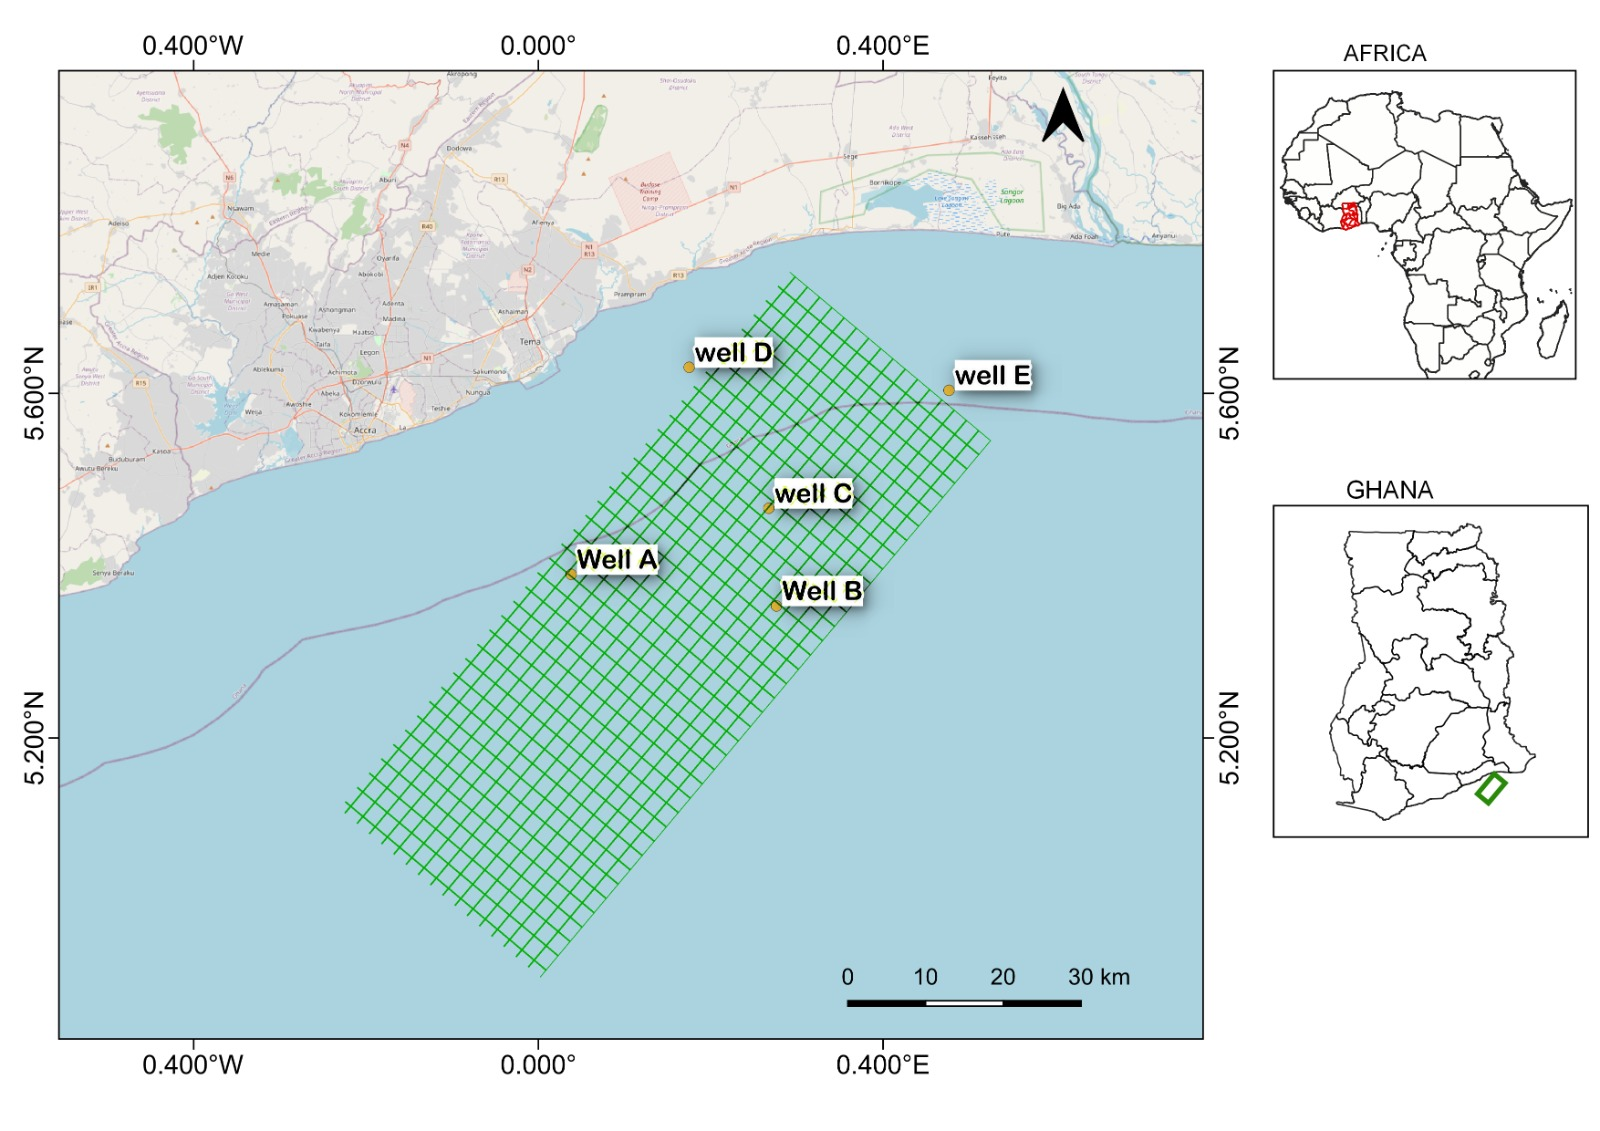
\includegraphics[width=\textwidth]{studyarea} % Replace with the actual filename and path of your figure
    \caption{Geographical position of Well-C in the offshore extension of the Keta Basin}
    \label{fig:study_area}
\end{figure*}
% \FloatBarrier

The Keta Basin stands as one of Ghana's four sedimentary basins, positioned among three offshore basins alongside Tano, Saltpond, and the onshore Voltaian basin \citep{lambon2020}.
Encompassing an area of approximately $33900$ sq. km, with 1900 sq. km on land, the basin is predominantly offshore, situated along the eastern expanse of the Ghanaian coast.
Bounded by the Chain Fracture Zone to the east and the Romanche Fracture Zone to the west, the structural confines of the Keta Basin contribute to its unique geological characteristics.
In contrast to the extensively explored Tano Basin, the Keta Basin has witnessed comparatively fewer exploration activities, despite its significant potential as part of the wider Gulf of Guinea Province. 
Both the Tano and Keta basins share a common geological origin, arising from tectonic activities during the final separation of South America from Africa \citep{falufosi2021geology}.
This shared origin implies similar sediment sources, suggesting that the Keta Basin holds promise as a potential source of commercial hydrocarbons.
The basin's geological underpinning comprises Precambrian basement rocks, followed by pre-rift sediments, primarily originating from the Triassic and Jurassic eras.
Noteworthy geological features include local syn-transform faults and substantial erosion, indicative of the regional syn-transform event that led to the separation of South America and Africa, removing over $3000$ m of material from the basin. 
The Cretaceous strata, serving as both source and reservoir rocks, represent the focal point for hydrocarbon exploration in the basin.
The Keta Basin also constitutes the western segment of the Dahomeyan embayment, extending into Togo, Benin, and parts of Nigeria. 
The basin's geological history spans from Precambrian sequences in the pre-rift stage through Tertiary sequences in the post-rift period, affirming its geological maturity and potential for hydrocarbon production \citep{akpati1978geologic}.
In summary, the Keta Basin, with its distinctive geological attributes and relatively unexplored nature, emerges as a promising frontier for hydrocarbon exploration within the Gulf of Guinea Province.
The basin's diverse geological history, ranging from Precambrian origins to Tertiary sequences, underscores its potential as a source of commercial hydrocarbons.

The Keta Basin spans both onshore and offshore regions. 
Our study specifically focuses on the offshore extension of the Keta Basin, situated within the geographical coordinates of latitudes \(3.35^\circ 42'2''\) to \(6.12^\circ 39'84''\) and longitudes \(-0.45^\circ 48'35''\) to \(2.0^\circ 00'61''\). 
Fig. \ref{fig:study_area} visually depicts the location of the analyzed Well-C within this offshore extension.

\section{Methods}\label{sec:methods}

The dataset used in the comprehensive analysis comes solely from the well logging of Well-C, which is strategically located in the eastern basin.
 This dataset contains important petrophysical logs namely the gamma-ray log (GR), shallow and deep resistivity log, neutron log (NPHI), and density log (RHOB).
 The logs summarized in Fig.\ref{fig:petroanaly1}  below were acquired within specified interest periods ranging from $1340$ m to $3060$ m.
%
\begin{figure*}%[htbp!]
    \centering    
    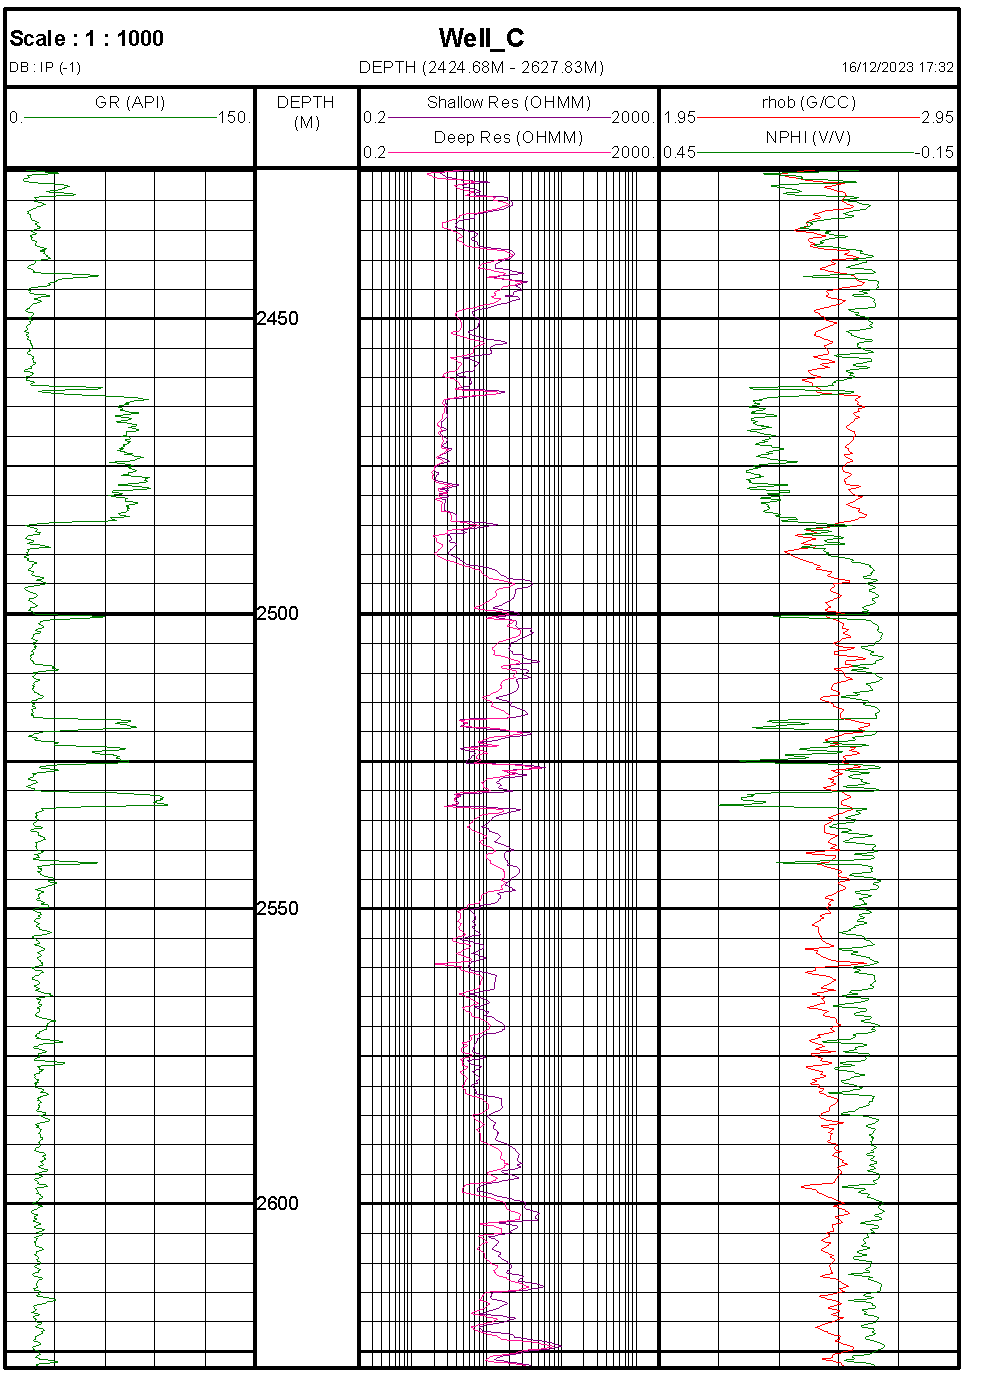
\includegraphics[width=0.9\textwidth]{Plogs} % petroanaly1  
    \caption{A spectral profile illustrating the Well-C logs, including gamma, resistivity, and density/ neutron, utilized in the petrophysical analysis.}    \label{fig:petroanaly1}
\end{figure*}
%
In Fig.~\ref{fig:petroanaly1}, each log plot exhibits a spectrum of values ranging from low to high, with each plot conveying distinct characteristics of the subsurface. 
The gamma-ray log serves the crucial purpose of distinguishing between shale and non-shale regions within the wellbore.
Meanwhile, the resistivity log plays a pivotal role in delineating fluid types in the subsurface, enabling the differentiation between brine, freshwater, and hydrocarbons. 
This discrimination is based on the conductivity properties, as brine is a superior conductor compared to freshwater, and hydrocarbons exhibit non-conductive behaviour.
The density log, owing to variations in the densities of different lithologies, becomes instrumental in distinguishing between diverse rocks in the subsurface, leveraging their distinctive bulk densities.
Additionally, the neutron log measures the presence of hydrogen atoms, providing insights into porosity.
When coupled with the density log, this tandem facilitates the discrimination between oil, gas, and water, contributing to a comprehensive understanding of the subsurface composition.
For the execution of this study's petrophysical analysis, the {\tt Schlumberger Interactive Petrophysics software version 3.5} was employed.
This sophisticated software not only facilitates the plotting of logs but also enables the generation of informative graphs.
The utilisation of such advanced software ensures a robust and accurate interpretation of the petrophysical data, thereby enhancing the reliability of the findings presented in this study.

\subsection{Lithology Identification} \label{subsec:Lithology}

Lithology identification serves as the foundational step in petrophysical analysis, as subsequent computations rely heavily on the type of lithology encountered \citep{akinyokun2009well}. 
In the context of the Keta Basin, an extensive review of the literature reveals a prevalent composition of shales, sandstones, and siltstones, with minor occurrences of limestones and conglomerates \citep{brownfield2006geology}.
Acknowledging this geological diversity, the gamma-ay log emerges as a powerful tool for lithological identification, given its effectiveness in differentiating between shale and non-shale zones within boreholes.
The gamma-ray log capitalises on naturally occurring radioactivity stemming from geological strata passed by boreholes, primarily sourced from isotopes such as uranium, thorium, and potassium-40  \citep{asfahani2021radioactivity}.
Widely utilized in the petroleum industry, the gamma-ray log plays a pivotal role in the analysis of lithology, calculation of shale volume, and examination of depositional environments \citep{mondol2015well}.
Moreover, it proves invaluable in inferring depositional facies and environments.
Notably, regions with low gamma-ray readings denote sand zones, while those with high gamma-ray readings signify shale zones.
Complementing the gamma-ray log, the density-neutron plot emerges as another crucial tool for lithological identification in the wellbore. 
Neutron porosity, in conjunction with density, holds significance in formation evaluation, with common practices involving the integration of these logs through programs like the density-neutron cross plot and overlay. 
These integrated approaches facilitate the determination of porosity, lithology, and the identification of gas-containing zones \citep{rodriguez2009new}.
The critical measurements obtained from the density and neutron logs are pivotal in the overall evaluation of formations.
The theoretical derivations linking hydrogen presence in sedimentary strata have strengthened the relationship between density and neutron logs, making them indispensable in contemporary assessment procedures.
Drawing on the work of \citep{mao2001physical}, the density-neutron plot provides key insights into porosity, lithology recognition, and the identification of natural gas formations.
A schematic representation of various lithologic interpretations in the well, as proposed by \cite{mondol2015well}, is adopted to visually elucidate the intricacies of the lithological analyses.

\begin{figure} %[htbp!]
    \centering    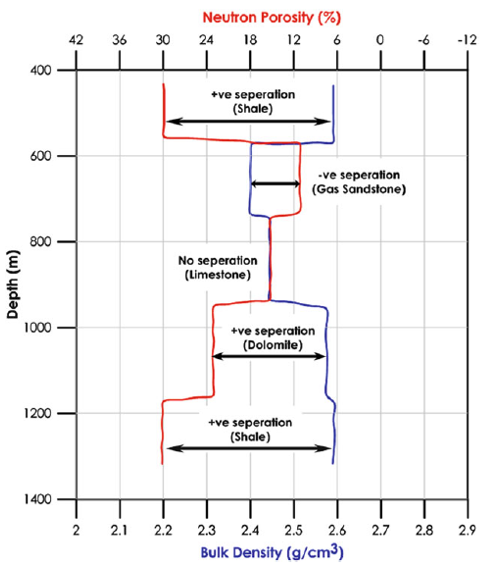
\includegraphics[width=\linewidth]{neutronporo} 
    \caption{Density/Neutron log responses illustrating variations in Shale, Dolomite, Limestone, and Gas Sandstone. Adopted from \cite{mondol2015well}.}
    \label{fig:neutronporo}
\end{figure}

\subsection{Delineation of reservoir zone} \label{subsec:reservoir}

In the overall structure of the petroleum system, the reservoir is the only component that is of the highest economic significance. Its ability to gather, hold, and then release hydrocarbons into the subsurface is what makes it significant. 
The porosity of the rocks that make up the reservoir is essential for efficient storage because it allows hydrocarbons to be retained in large quantities.
According to \cite{oyeyemi2018hydrocarbon}, the reservoir must also be permeable, adequately thick, and widely spread in order to be commercially viable. 
Sandstones and carbonates are excellent alternatives for reservoir formations since they fit these requirements well.

One of the most important jobs in reservoir studies is identifying and delineating reservoir zones.
During this process, the gamma-ray log and the deep resistivity log are essential tools. 
Zones that are identified as gross Reservoir zones are those that have low gamma-ray readings and high resistivity values (more than $10$ ohms). 
This combination method helps prevent misclassifications, especially in situations where sands with high radioactive mineral concentrations could be mistakenly classified as shales \citep{lai2023typical}.
The critical roles of porosity and permeability must be emphasised to expound on reservoir characterisation. 
The porosity of the reservoir, as shown by well logs like the Neutron log, indicates that there are gaps in the rock formation. 
Sufficient porosity is essential for holding and tolerating large amounts of hydrocarbons.
In addition, how easily hydrocarbons can travel across the reservoir is determined by permeability, a measure of the rock's fluid-transmitting capacity.
The reservoir's overall commercial viability is greatly influenced by both variables.


\subsection{Shale volume calculation} \label{subsec:Shale}
The quantification of clay content in a reservoir is a critical parameter for reservoir evaluation, influencing its overall quality.
Shale, which contains a significant amount of clay, serves as an indicator of reservoir characterisation. 
A higher shale volume can be indicative of a less favourable reservoir, while a lower shale volume suggests the presence of more sands, signalling a potentially better reservoir quality. 
In this study, the calculation of shale volume employed the linear gamma-ray equation, a well-established method for assessing the clay content in subsurface formations.
The shale volume parameter plays a multifaceted role in reservoir analysis.
Firstly, it contributes to the determination of the gross thickness of the reservoir, providing insights into the overall thickness, inclusive of shale components.
Additionally, shale volume is integral to the calculation of porosity, a crucial factor in assessing the reservoir's capacity to hold hydrocarbons.
Furthermore, it is a key parameter in the computation of water saturation, influencing the distribution and mobility of hydrocarbons within the reservoir \citep{szabo2013extending}.

The presence of shale, whether in the form of particles, minerals, or thin laminae, directly impacts the amount of moveable hydrocarbons within the reservoir.
As shale volume increases, the permeability of the reservoir may decrease, affecting the flow of hydrocarbons.
This study utilized a linear approximation for shale volume, employing a 45\% shale cutoff to delineate the threshold for categorising shale content.
It is essential to recognize the interconnected nature of shale volume with other fundamental reservoir parameters. 
The linear approximation method used in this study, with the specified shale cutoff, enhances the precision of shale volume calculations and contributes to a more accurate understanding of reservoir characteristics.

\begin{equation}\label{eq:sh}
    V_{\text{sh}} = {\rm \frac{GR-GR_{min}}{GR_{max} - GR_{min}}},
\end{equation}

\noindent where \( V_{\text{sh}}\) is the volume of shale,
 \( \text{GR} \) is the gamma-ray value at a specific depth in the well log, \( \text{GR}_{\text{min}} \) is the minimum gamma-ray value in the log (typically associated with clean, non-shale intervals), and \( \text{GR}_{\text{max}} \) is the maximum gamma-ray value in the log (typically associated with high shale content).

\subsection{Fluid type and contact Identification} \label{subsec:fluid}

Identifying reservoir fluids is a critical aspect of subsurface characterisation, with deep-resistivity logs and density neutron logs serving as key tools in this process.
The deep-resistivity log is particularly valuable as it measures the uninvaded zone of the well, providing a record of the true resistivities of the rocks encountered. Given that hydrocarbons are non-conductive, an expectation arises that in the presence of hydrocarbons, the recorded resistivity values should be elevated. 
Typically, resistivity values of $10$ ohms and higher are expected in such scenarios.
Moreover, the crossover between density and neutron logs plays a pivotal role in distinguishing between different reservoir fluids, namely oil, gas, and water.
The crossover phenomenon is especially pronounced in the presence of gas, resulting in the widest separation between the logs. 
In contrast, a narrower crossover is anticipated in the presence of oil, and when water is present, the two logs exhibit proximity, as visually depicted in Fig.~\ref{fig:shale} below.
It illustrates the distinct crossovers associated with different fluid types, providing a visual representation of the log responses in varying reservoir conditions.
The identification of specific fluid contacts is crucial to understanding reservoir dynamics.
The interface between gas and oil is termed the gas-oil contact; the boundary between oil and water is known as the oil-water contact; and in situations where oil is absent, the contact between gas and water is referred to as the gas-water contact.

This intricate interplay of log responses and fluid contacts contributes significantly to the reservoir characterisation process.
By leveraging the information derived from deep-resistivity, density, and neutron logs, exploration and production teams can make informed decisions regarding the nature and distribution of reservoir fluids, thereby optimising reservoir development strategies and maximising hydrocarbon recovery.

\begin{figure}%[htbp!]
    \centering    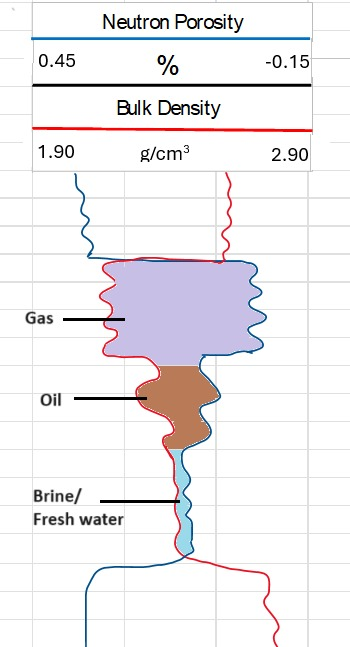
\includegraphics[width=\linewidth]{dolomite} %shale
    \caption{Cross-plot illustrating the interpretation assigned to different fluid signatures based on Density and Neutron logs.}
    \label{fig:shale}
\end{figure}

\subsection{Porosity and Water Saturation Calculations} \label{subsec:porosity}

To assess both porosity and water saturation in subsurface formations, key logs such as the gamma-ray log, neutron log, density log, and the calculated volume of shale are employed.
The neutron log, in conjunction with density, holds significance in formation evaluation. 
Commonly, these logs are amalgamated in software applications, like the density-neutron crossplot and overlay, to derive comprehensive insights into porosity, lithology, and the presence of gas-containing zones.
Such integrated analyses play a crucial role in making informed decisions during reservoir evaluation.
Porosity, a fundamental parameter for reservoir characterisation, is typically derived from Neutron and Density logs. 
A minimum porosity value of 10\% is considered a threshold for making economically viable decisions.
The calculation of porosity involves intricate equations that take into account various log measurements.
Water saturation, another crucial aspect of reservoir evaluation, is also determined through a dedicated equation.
The utilisation of the gamma-ray log aids in identifying shale content, contributing to the calculation of the volume of shale, which is an integral component in porosity and water saturation calculations.
The synergy of these logs enables a comprehensive understanding of the subsurface, guiding decision-making processes in hydrocarbon exploration and production.
The mathematical expressions of porosity and water saturation are defined by Eqs.~\eqref{eq:por} and \eqref{eq:sw}, respectively:

 \begin{equation}\label{eq:por}
 \phi = \frac{{\text{Neutron Porosity}}}{{1 - \text{Volume of Shale}}} \end{equation}
 
\begin{equation}\label{eq:sw} S_w = \frac{{\text{Density - Neutron Porosity}}}{{1 - \text{Volume of Shale}}}\end{equation}

\noindent These equations serve as foundational tools in reservoir evaluation, providing quantitative measures for critical parameters.
The incorporation of the volume of shale acknowledges the impact of shale content on porosity and water saturation calculations, enhancing the accuracy and reliability of the evaluation process.

\subsection{Net pay} \label{subsec:net}

The determination of net pay is a critical parameter in reservoir evaluation that relies on the integration of shale volume, porosity, and water saturation with predefined cutoff values as reported in Table~\ref{tab:net_pay_cutoffs}.
In this study, specific cutoff criteria were established to delineate reservoir zones effectively.
The predetermined cutoffs included a shale volume cutoff of 45\%, a porosity cutoff of 10\%, and a water saturation cutoff of 65\%.
These thresholds serve as pivotal benchmarks in characterising the reservoir and delineating zones with favourable hydrocarbon potential.

\begin{table*}%[htbp]
    \centering
\caption{Cutoff values utilized for net pay zone calculation} \label{tab:net_pay_cutoffs}
    \begin{tabular}{|p{4cm}|p{3cm}|p{4cm}|}
        \hline
        \textbf{Petrophysical parameter} & \textbf{Equation for cutoff} & \textbf{Zone label after cutoff} \\
        \hline
        Volume of shale (\(V_{\rm sh}\)) &  \(0\% \leq V_{\rm sh} \leq 45\%\)\quad & Net sand \\
        \hline
Volume of shale (\(V_{\rm sh}\)) and porosity (\( \phi\)) & \(0\% \leq V_{\rm sh} \leq 45\%\)\quad \(10\% \leq \phi \leq 50\%\) 
         & Net reservoir\\
        % Add more rows as needed
        \hline
Volume of shale (\(V_{\rm sh}\)), porosity (\( \phi\)), and water saturation (\(S_w\)) & \(0\% \leq V_{\rm sh} \leq 45\%\)\quad \(10\% \leq \phi \leq 50\%\) \quad
        \(0\% \leq S_{\rm w} \leq 65\%\)\quad & Pay zone\\
        % Add more rows as needed
        \hline
    \end{tabular}
\end{table*}
%
The shale volume cutoff is crucial in identifying intervals with elevated clay content, which could impact reservoir quality. 
The porosity cutoff ensures that only zones with sufficient pore space for hydrocarbon storage are considered, with a minimum value of 10\% set as a baseline for economic viability.
Simultaneously, the water saturation cutoff of 65\% serves as an indicator of the presence of movable hydrocarbons, aiding in the determination of reservoir quality.
These predetermined cutoff values streamline the analysis process, facilitating the identification of net pay zones within the subsurface. 
The utilisation of such thresholds enhances the precision of reservoir characterisation, guiding decision-making processes in resource exploration and development.

\section{Results and Discussion} \label{sec:RnD}

\subsection{Lithology and reservoir identification } \label{subsec:reserv}

The analysis of well logs, specifically the gamma-ray, resistivity, and density logs, has facilitated the identification and characterisation of the reservoir zones within Well-C.
The logs collectively reveal the predominant presence of sandstones, accompanied by intermittent traces of limestones.
To further refine the lithological understanding of the reservoir, the Schlumberger neutron density cross-plot (refer to Fig.~\ref{fig:sand123}) was employed. 

The areas highlighted by rectangular demarcations in the neutron density plots (refer to Figs.~\ref{fig:sand1} and~\ref{fig:sand2} ) represent sand formations with the occurrence of gas. 
These sands exhibit bulk densities ranging from $2.2$ to $\rm 2.4 gm/cc$ and are characterised by low neutron values. 
The trend is consistently observed throughout the reservoir regions, except for Sand $3$ (refer to Fig.~\ref{fig:sand3}), where the absence of gas is evident, showcasing the exclusive presence of water.
Conversely, the regions delineated by circular markers on the plots (refer to Figs.~\ref{fig:sand1}--~\ref{fig:sand3} ) demonstrate escalating densities within the range of $2.45$ to $2.56$ gm/cc, accompanied by a corresponding decline in neutron porosity values. 
This phenomenon suggests the presence of water and/ or cementitious materials, contributing to higher density readings and indicating a compact nature of the sands in these areas.
The disparity in density is attributed to the inherent differences between water and gas, with water being denser.
Consequently, the water-dominated regions exhibit higher density values compared to the gas-dominated areas. This consistent pattern is observable across all three reservoir regions examined in the study.

By examining the depth information extracted from the logs, which spans approximately 2430--2630 m, it has been determined that the reservoir spans the upper lower Cretaceous and early upper Cretaceous periods (refer to Fig~\ref{fig:perto2}.
This temporal context aligns with literature findings, associating these geological intervals with the presence of sandstones and shaley sandstones, commonly linked to marine deposits \citep{brownfield2006geology}.
Notably, this period coincides with the conclusion of the syn-transform, marked by geological phenomena such as block faulting, graben filling, and basin extension.
The identification of the reservoir was further substantiated by the observation of relatively higher porosities, elevated resistivity values, and distinctive density neutron crossovers.
In summary, Fig.~\ref{fig:perto2} illustrates the demarcation of three distinct reservoir units.
The first, denoted as Sand $1$, exhibits a gross thickness of $37.64$ m, while the second, labelled Sand $2$, boasts a gross thickness of $31.39$ m. 
The third unit, designated as sand three, presents a substantial gross thickness of $95.25$ m.
The cumulative reservoir thickness, obtained by aggregating the intervals of these three sand units, amounts to $164.28$ m.
Importantly, shale units intercalated between the sands act as barriers, influencing the reservoir architecture by creating distinct compartments within the geological formation.


\begin{figure*}
\centering
\begin{subfigure}{0.4\textwidth}
    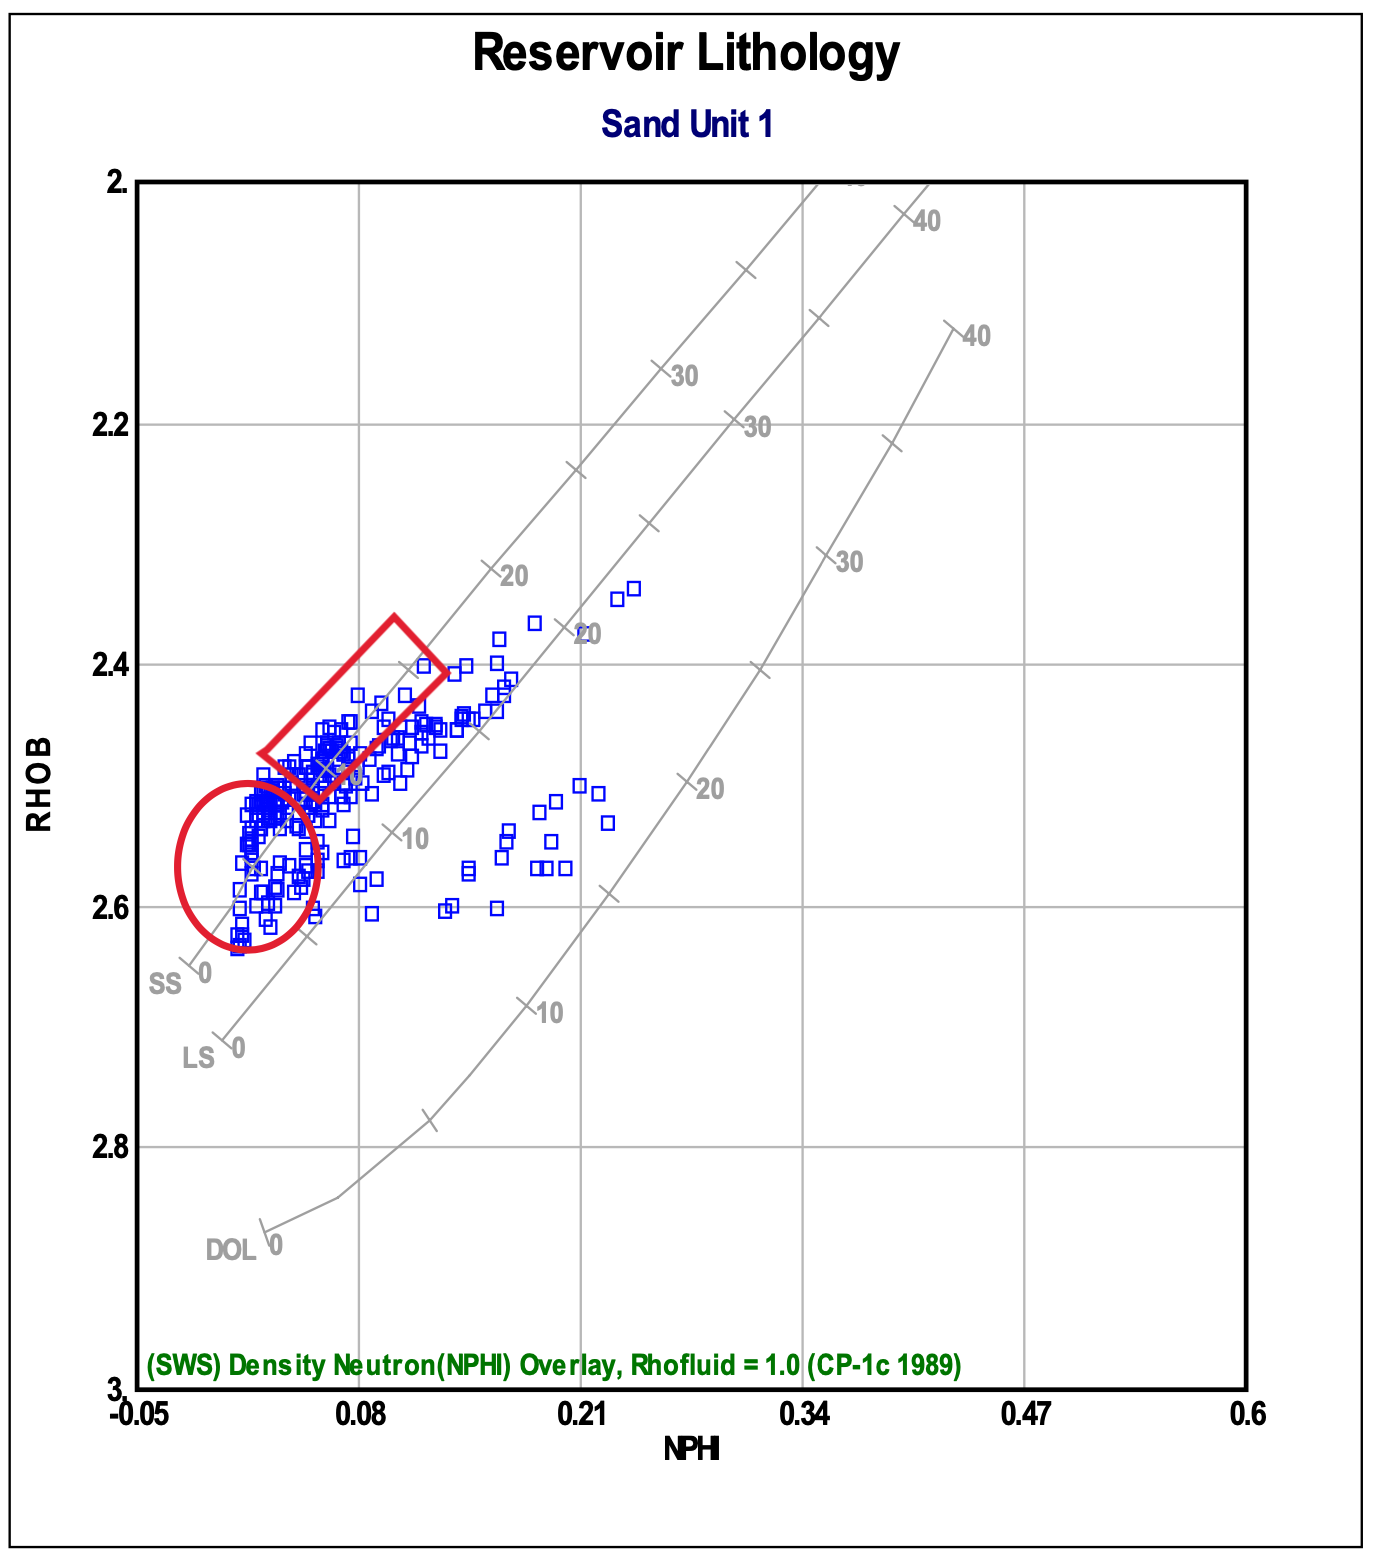
\includegraphics[width=\textwidth]{SS1} %sand1
    \caption{Sand 1}
    \label{fig:sand1}
\end{subfigure}
\hfill
\begin{subfigure}{0.4\textwidth}
    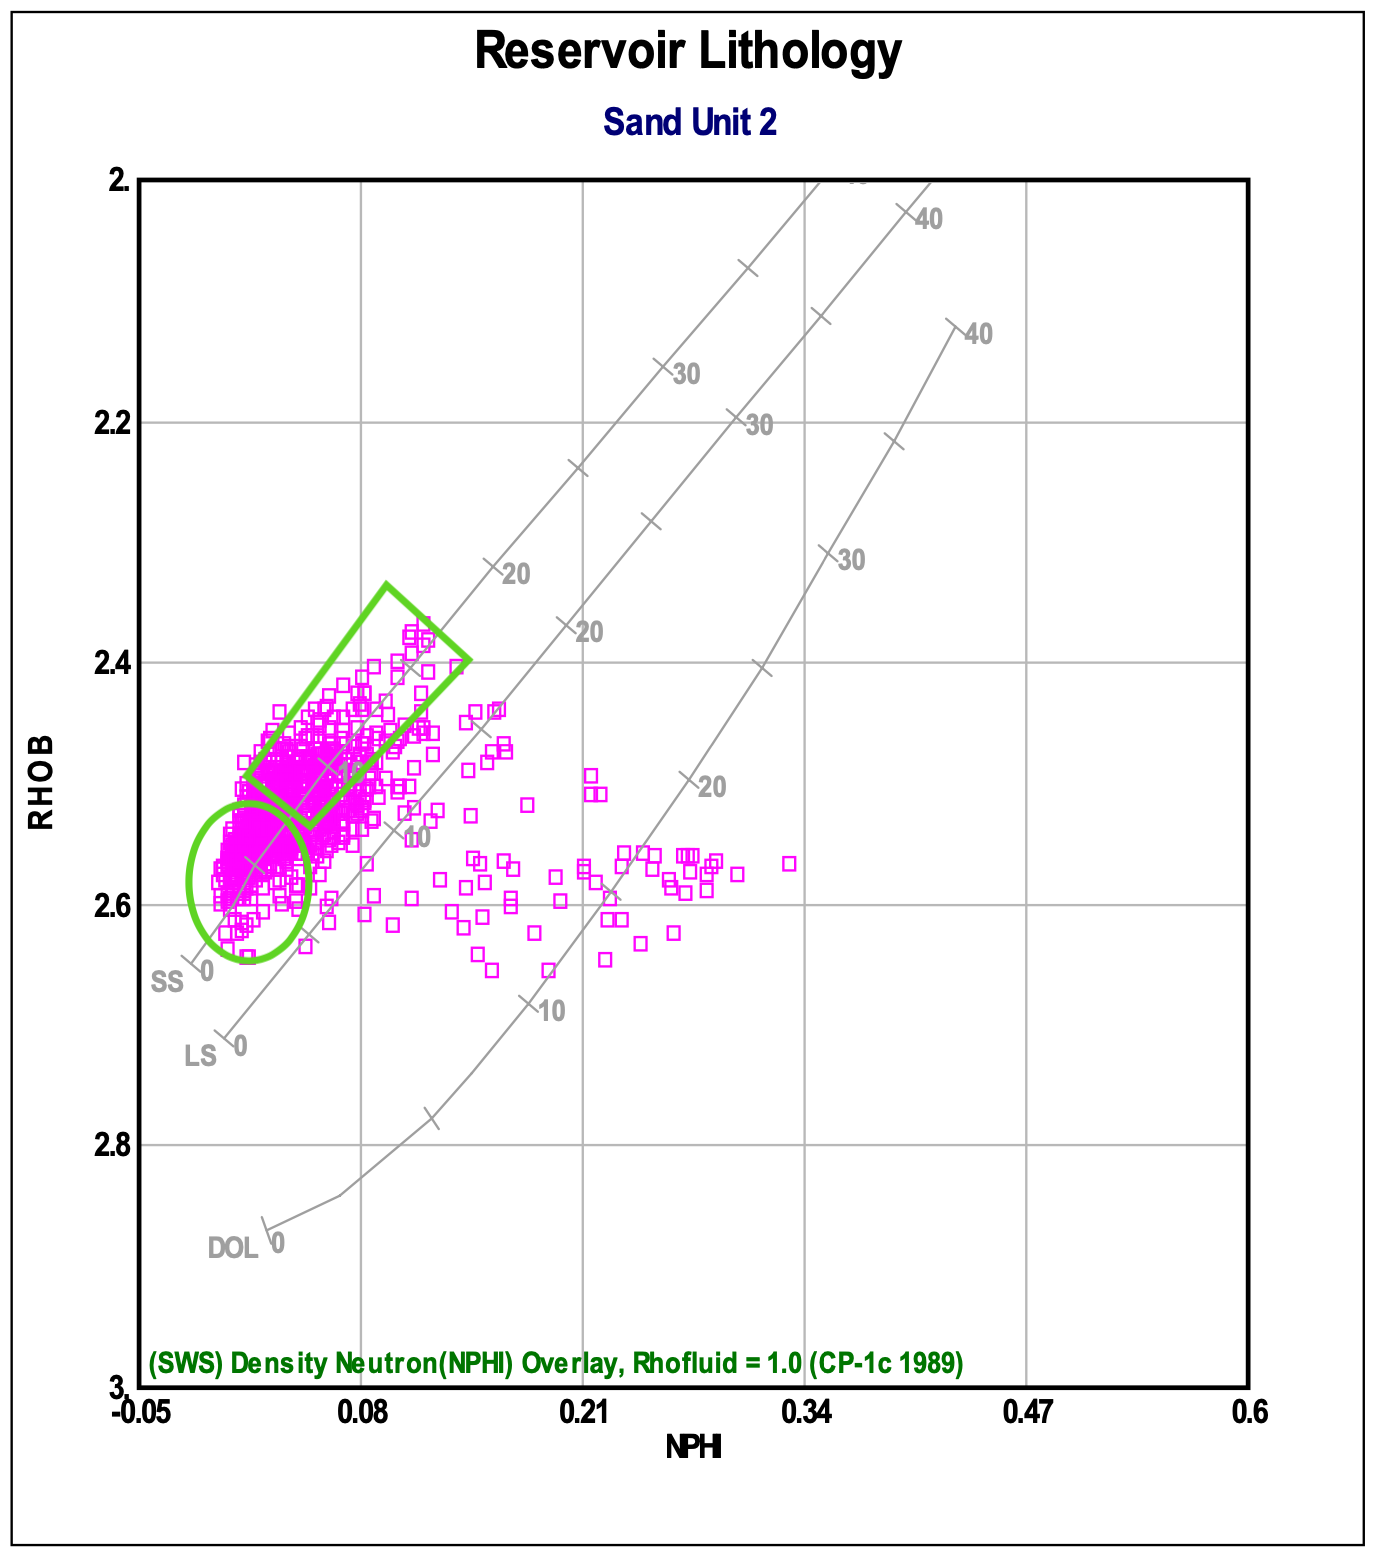
\includegraphics[width=\textwidth]{SS2}
    \caption{Sand 2}
    \label{fig:sand2}
\end{subfigure}
\hfill
\begin{subfigure}{0.4\textwidth}
    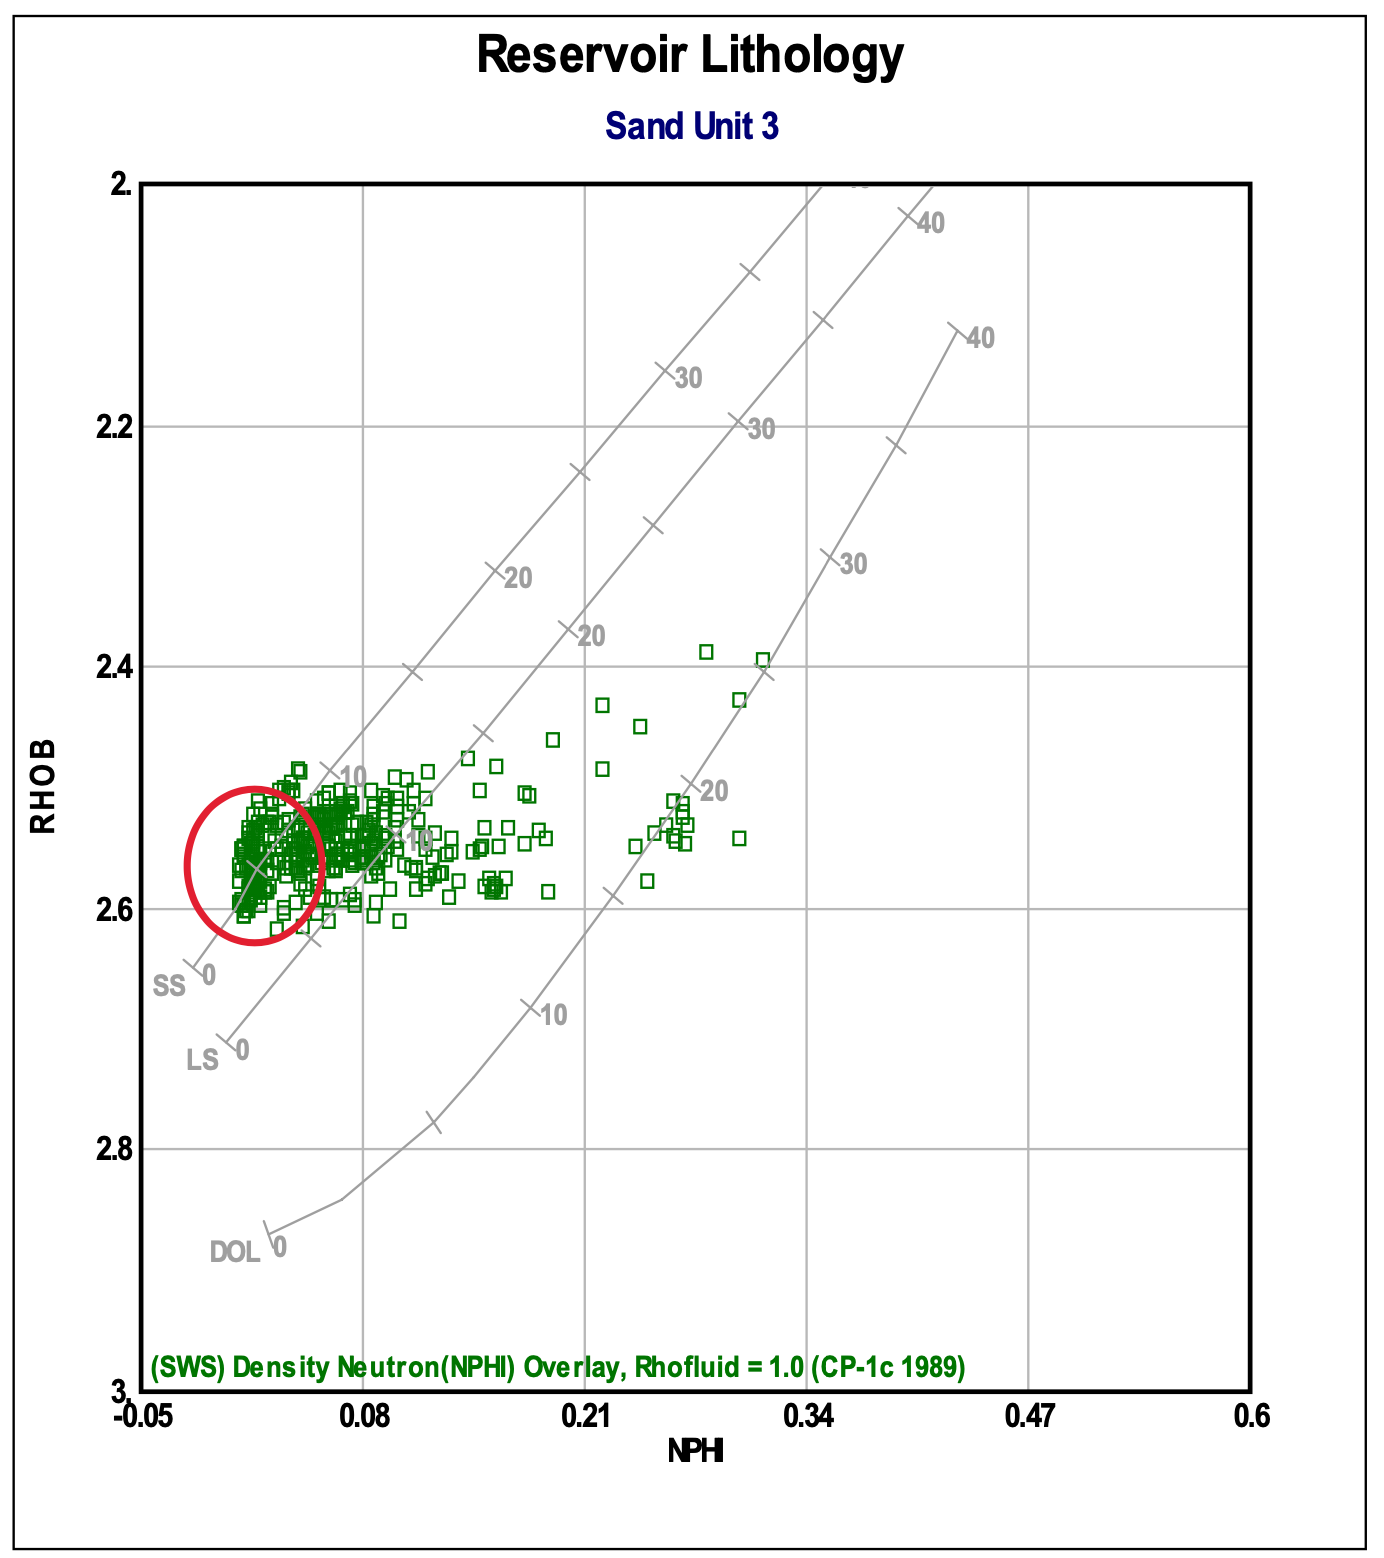
\includegraphics[width=\textwidth]{SS3}
    \caption{Sand 3}
    \label{fig:sand3}
\end{subfigure}
        
\caption{RHOB-NPHI Crossplot of Sand Units in Well-C: (a) Sand $1$, (b) Sand $2$, and (c) Sand $3$, illustrating their lithologic composition.}\label{fig:sand123}
\end{figure*}

%
\begin{figure*}%[htbp!]
    \centering    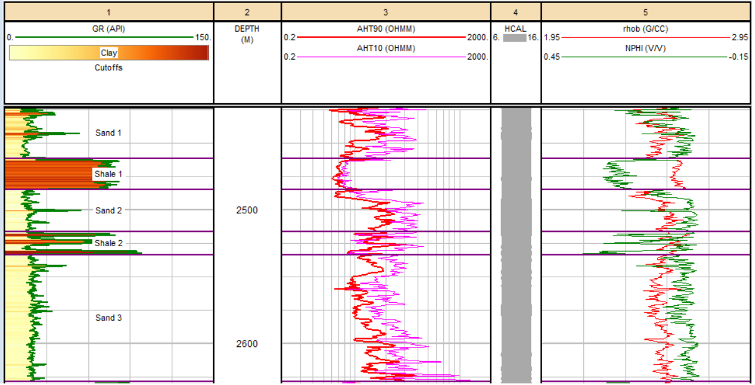
\includegraphics[width=0.9\textwidth]{perto2}%{pdfs/Plogs} 
    \caption{Reservoir units in Well-C: Sand $1$ Sand $2$, and  Sand $3$ are identified and labelled within the geological formation.}
    \label{fig:perto2}
\end{figure*}
% %

\subsection{Fluid identification } \label{subsec:Rfd}

Identification of the fluids within the delineated reservoir zone was accomplished through the analysis of the density-neutron cross plot. 
Following established practices and literature findings, the interpretation of the cross plot is grounded in the distinct characteristics exhibited by different fluids. 
A broader crossover of the density-neutron logs is commonly indicative of gas, a more confined crossover is associated with oil, and the most constrained crossover is attributed to water.
Fig.~\ref{fig:petro3} illustrates the manifestation of all three fluids within the reservoir.
While both oil and gas have been identified within the three demarcated reservoir zones, it is essential to emphasize that the prevailing hydrocarbon within this geological formation is predominantly gas.
This distinction is critical in understanding the composition of the hydrocarbon reserves and has significant implications for further exploration and extraction strategies. 
The comprehensive identification of fluid types within the reservoir enhances the reservoir characterisation process and contributes valuable insights to guide subsequent decision-making processes in hydrocarbon exploration and production.
%
%
% \clearpage
\begin{figure*}%[htbp!]
    \centering    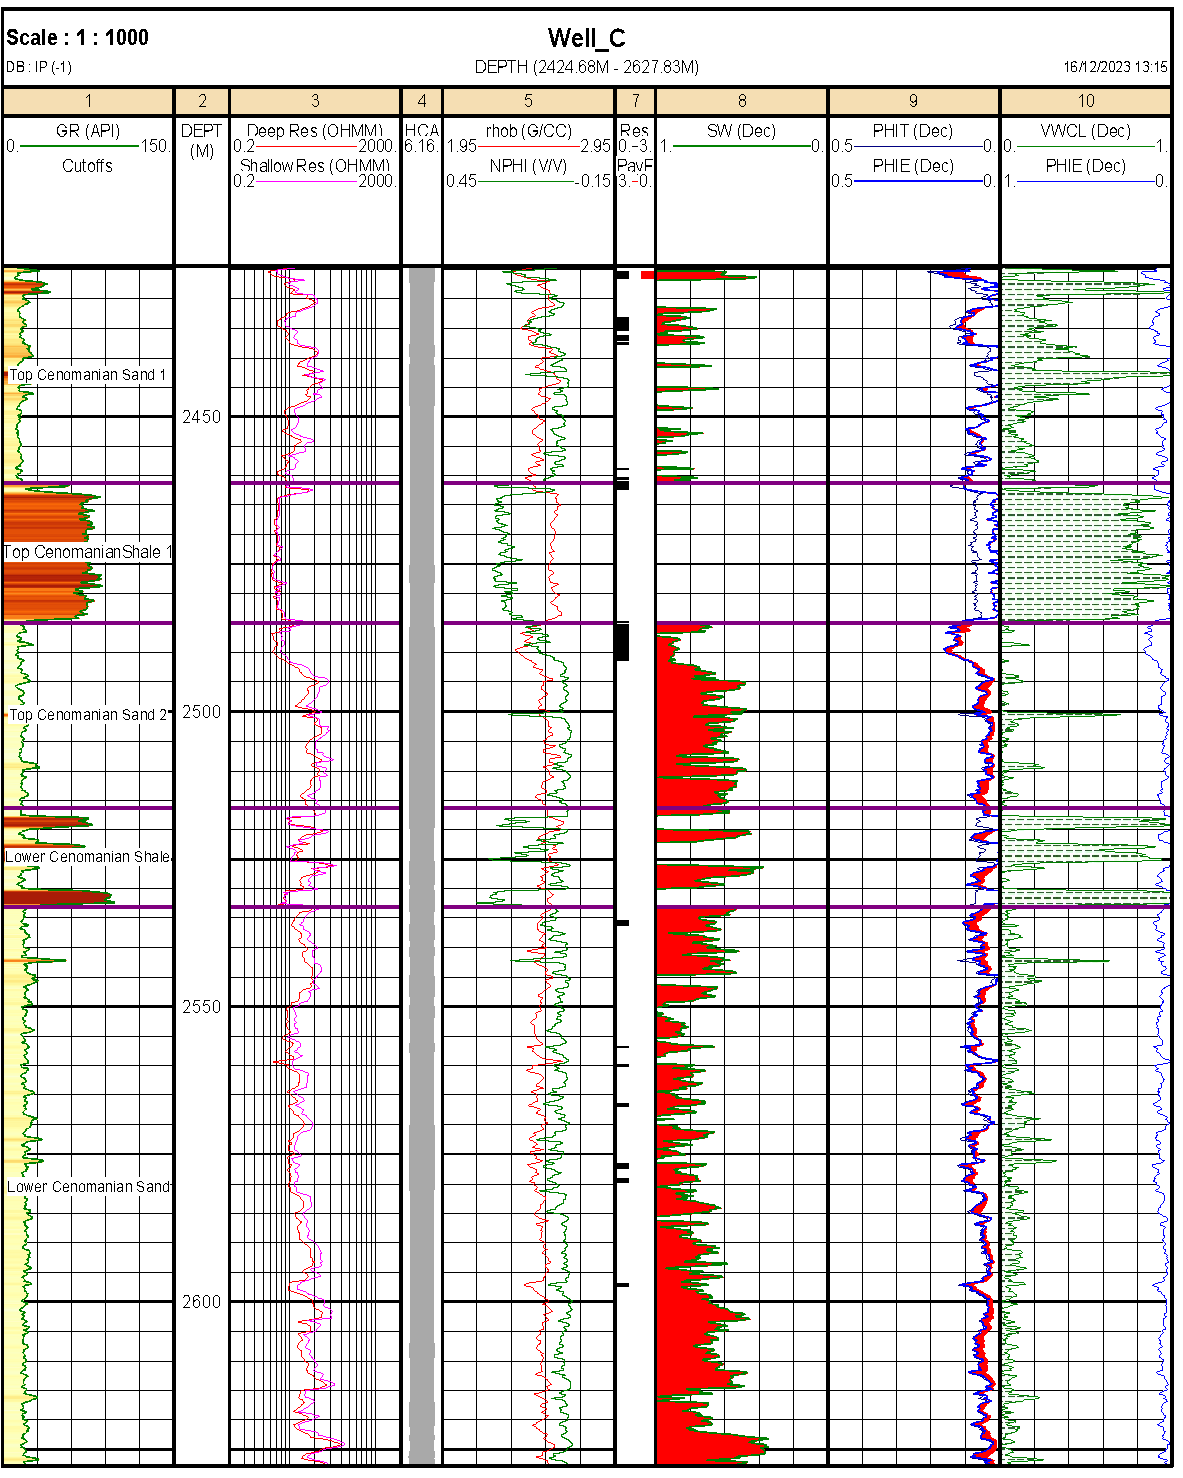
\includegraphics[width=\textwidth]{GP} %final_general
   \caption{Illustration of composite log response and lithology interpretation of the hydrocarbon-bearing zone depicted along the interval depth in Keta Basin Well-C.}\label{fig:petro3}     
\end{figure*}
%
%
\begin{table*}%[htbp]
    \centering
    \caption{Petrophysical parameter estimation}
    \label{tab:params}
    \begin{tabular}{|c|c|c|c|c|c|c|c|}
        \hline
        \textbf{Zones} & \textbf{Top} & \textbf{Bottom} & \textbf{Gross thickness} & \textbf{Net thickness} & \textbf{Av. \(\rm V_{sh}\)} & \textbf{Av. \(\rm \phi\)} & \textbf{Av. \(\rm S_w\)} \\
        \hline
        % Add your table content here
        Top Cenomanian Sand 1 & 2423.62 & 2461.26 & 37.64 & 4.57 & 0.183 & 0.123 & 0.733 \\
        \hline
        Top Cenomanian Sand 2 & 2484.88 & 2516.28 & 31.39 & 6.1 & 0.024 & 0.132 &  0.861\\
        \hline
        Lower Cenomanian Sand  & 2533.04 & 2628.29 & 95.25 & 3.05 & 0.062 & 0.106 &  0.721\\
        \hline
    \end{tabular}    
\end{table*}
%
According to the data presented in Table~\ref{tab:params}, the total gross depth of the reservoir is determined to be $164.28$ m, yet only a relatively limited section of approximately $13.72$ m contains detectable hydrocarbons.
This volume falls significantly below the threshold considered economically viable for drilling operations.
Given the relatively low proportion of hydrocarbon-bearing intervals within the overall reservoir depth, there are concerns about the economic feasibility and potential profitability of drilling activities in this geological formation.
Further evaluation and strategic considerations are warranted to determine the most prudent course of action in light of these findings.

\section{Conclusion} \label{sec:conc}

Upon the application of all the designated cutoffs for net pay determination, it became evident that two out of the three initially identified reservoir sands lack hydrocarbon potential. Despite being categorized as sands, these regions exhibit such low porosities that render them unviable for conventional hydrocarbon production methods.
The term "tight sands" is attributed to these formations, indicating a scarcity of pore spaces crucial for hydrocarbon mobility. 
This diminished porosity is attributed to overcompaction resulting from deep burial depths over geological time.

Contrastingly, the first reservoir sand recognized, namely Top Cenomanian Sand 1, exhibits a porosity above the established cutoff of $0.8$, suggesting the potential for gas production from this reservoir. 
However, it is noteworthy that the cumulative depth of both net reservoir and net pay in Top Cenomanian Sand 1 amounts to a mere $2.0$ m.
Such a shallow depth raises economic concerns, as investing significant financial resources for production becomes impractical given the limited resource volume.

Therefore, the prospect of revisiting the Cenomanian sands in the Keta Basin is suggested, albeit with a shift toward unconventional methods. Reevaluating these formations with unconventional approaches might offer alternative strategies for optimising hydrocarbon recovery.
The need for innovative techniques and technologies becomes apparent in the quest to unlock the potential of these reservoirs, considering their unique characteristics and limitations revealed through the application of cutoff criteria.
Further exploration and research are warranted to explore the viability of unconventional methods and potentially transform these seemingly nonproductive sands into economically viable hydrocarbon reservoirs.


\begin{acknowledgments}
The authors express their gratitude to GNPC for generously supplying the essential well-log data crucial to the success of this Ph.D research. 
Appreciation is extended to the Research Groups at the Earth Science Department, University of Ghana, and the Ghana Space Science and Technology Institute for their valuable insights and feedback. 
Special thanks from H. Adams to Ms. Caroline Edinam Doe's for recognising her assistance in creating the study area map.
\end{acknowledgments}

% \subsection{Data Availability}
% Data Availability after the Acknowledgments section and before the Appendices/References can be
% included with the \texttt{dataavailability} environment, as

% \begin{verbatim}
% \begin{dataavailability}
% The inclusion of a Data Availability Statement ...
% \end{dataavailability}
% \end{verbatim}


\begin{dataavailability}
Data supporting the findings of this study are available upon reasonable request. Requests for data should be addressed to the corresponding author.
While the original data generated during the course of the study is not publicly available, we are committed to providing access to the data upon request to ensure transparency and reproducibility of the research findings.
\end{dataavailability}




\bibliographystyle{gji}
\bibliography{cas-refs}


% \appendix
% \section{For authors}

% Table~\ref{authors} is a list of design macros which are unique to GJI. The
% list displays each macro's name and description.

% \section{For editors}

% The additional features shown in Table~\ref{editors} may be used for
% production purposes.

\bsp % ``This paper has been produced using the Blackwell
     %   Publishing GJI \LaTeXe\ class file.''

\label{lastpage}


\end{document}
